
\subsubsection{Meeting State Machine}
This State Machine was created with the purpose to identify the various states a meeting can be in and the show the transition events that modify its state.

\begin{figure}[htp] 

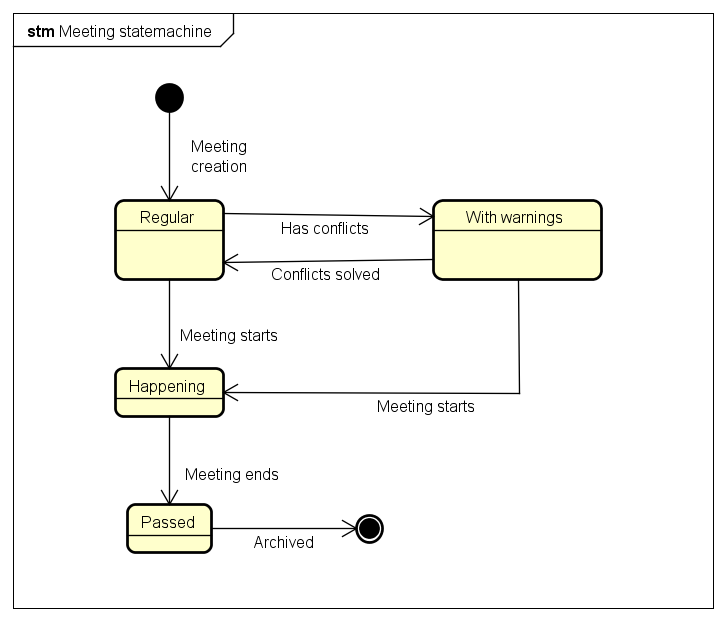
\includegraphics[width=\textwidth]{statecharts/meetingstatemachine} 
\caption{State Chart showing states of a meeting} 
\label{fig:meetingstatemachine} 
\end{figure} 

\newpage
\subsubsection{Basic UX State Chart}
We provide a simple and basic User Experience State Chart which highlights the different pages a user can find himself in (and the System redirects the user to, when an event happens). 
\\We believe this could be helpful to understand and visualize the entire application.

\begin{figure}[htp] 

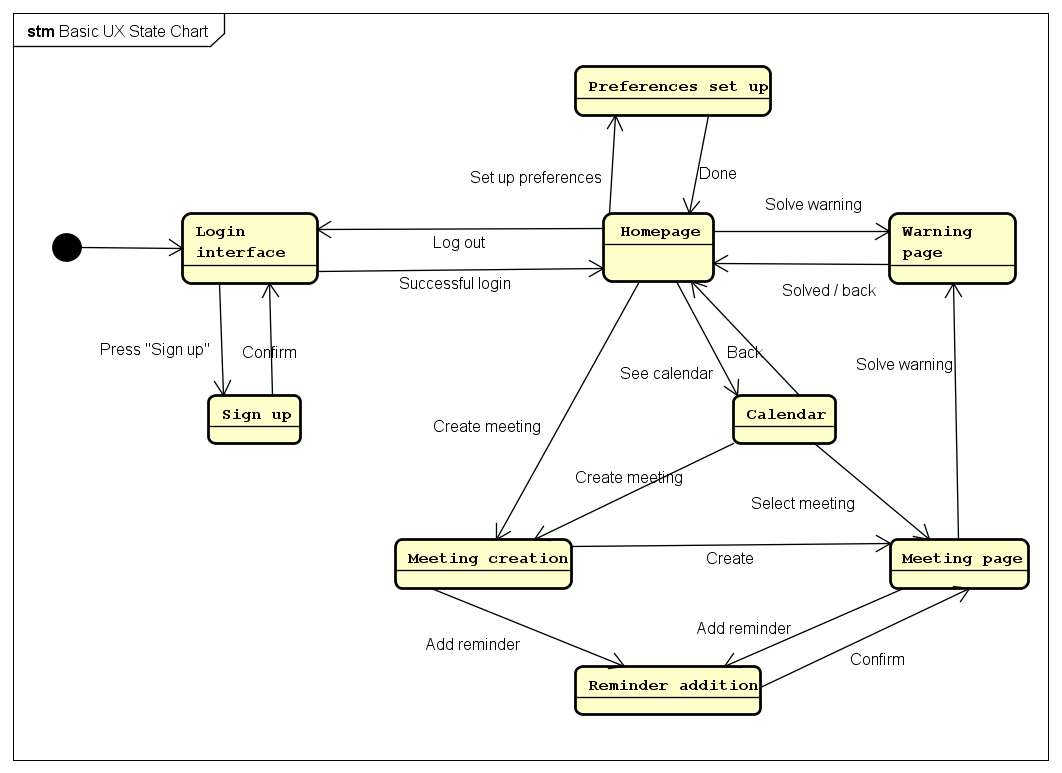
\includegraphics[width=\textwidth]{statecharts/basicux} 
\caption{A basic User eXperience chart of the application} 
\label{fig:ux} 
\end{figure}